\documentclass[10pt]{article}
\usepackage[margin=0.7in,top=0.5in,bottom=0.5in]{geometry}
\usepackage{booktabs,graphicx,amsmath,amssymb,enumitem,xcolor,titlesec,multicol}
\usepackage[hidelinks]{hyperref}
\usepackage[T1]{fontenc}\usepackage{lmodern}
\setlength{\parindent}{0pt}\setlength{\parskip}{2pt}
\titlespacing*{\section}{0pt}{5pt}{2pt}\titleformat{\section}{\large\bfseries}{\thesection.}{0.5em}{}
\titlespacing*{\subsection}{0pt}{4pt}{1pt}\titleformat{\subsection}{\normalsize\bfseries}{}{0em}{}
\setlist[itemize]{leftmargin=1.1em,itemsep=1pt,topsep=1pt,parsep=0pt}
\newcommand{\ganSRTr}{2.48}
\newcommand{\authSRTr}{3.02}
\newcommand{\lsSRTr}{1.98}
\newcommand{\ridgeSRTr}{1.77}
\newcommand{\uncSRTr}{1.52}
\newcommand{\ganSRVa}{1.29}
\newcommand{\authSRVa}{1.39}
\newcommand{\lsSRVa}{0.79}
\newcommand{\ridgeSRVa}{1.24}
\newcommand{\uncSRVa}{0.70}
\newcommand{\ganSRTe}{0.66}
\newcommand{\authSRTe}{0.77}
\newcommand{\lsSRTe}{0.42}
\newcommand{\ridgeSRTe}{0.49}
\newcommand{\uncSRTe}{0.45}
\newcommand{\tfSRTr}{2.58}
\newcommand{\tfSRVa}{1.34}
\newcommand{\tfSRTe}{0.73}
\newcommand{\nTrialsTf}{3}
\newcommand{\tfTeMin}{0.49}
\newcommand{\tfTeMax}{0.69}
\newcommand{\tfVaMin}{0.98}
\newcommand{\tfVaMax}{1.16}
\newcommand{\trialVaMin}{0.53}
\newcommand{\trialVaMax}{1.00}
\newcommand{\nTrials}{9}
\newcommand{\ganSRTeAnn}{2.3}
\newcommand{\authSRTeAnn}{2.7}
\newcommand{\trialTeMin}{0.15}
\newcommand{\trialTeMax}{0.63}
\newcommand{\authEVTe}{0.07}
\newcommand{\authXSTe}{0.21}
\newcommand{\authEVTr}{0.16}
\newcommand{\authXSTr}{0.13}
\newcommand{\ganEVTe}{0.06}
\newcommand{\ganXSTe}{0.22}
\newcommand{\ganEVTr}{0.17}
\newcommand{\ganXSTr}{0.14}
\newcommand{\tfEVTe}{}
\newcommand{\tfXSTe}{}
\newcommand{\tfEVTr}{}
\newcommand{\tfXSTr}{}
\newcommand{\lsEVTe}{0.03}
\newcommand{\lsXSTe}{0.15}
\newcommand{\ridgeEVTe}{0.03}
\newcommand{\ridgeXSTe}{0.15}
\newcommand{\turnDollar}{0.94}
\newcommand{\turnLong}{0.40}
\newcommand{\turnShort}{0.97}
\newcommand{\srNetTen}{0.57}
\newcommand{\srNetTwentyFive}{0.45}
\newcommand{\srNetFifty}{0.24}
\newcommand{\srEarly}{0.83}
\newcommand{\srLate}{0.47}
\newcommand{\srExGFC}{0.71}
\newcommand{\maxLoss}{-4.2}
\newcommand{\corrPortTe}{0.87}
\newcommand{\corrPortTr}{0.92}
\newcommand{\corrOursTe}{0.83}
\newcommand{\corrOursTr}{0.84}

\newcommand{\paper}{Chen, Pelger \& Zhu (2024)}

\begin{document}
\begin{center}
{\LARGE\bfseries Replicating \emph{Deep Learning in Asset Pricing}}\\[2pt]
{\normalsize Chen, Pelger \& Zhu, \emph{Management Science} 70(2), 2024 \quad---\quad MFE 230ZA final project}\\[1pt]
{\small Data, method, challenges and extensions of a from-scratch PyTorch replication of the GAN stochastic discount factor}
\end{center}
\vspace{-4pt}

\section{Data}
\textbf{What the paper uses.} Monthly CRSP excess returns for all US stocks with a complete set of 46 firm characteristics
(past returns, investment, profitability, intangibles, value, trading frictions), January 1967 -- December 2016.
Characteristics are rank-transformed cross-sectionally every month into $[-0.5,0.5]$. The macro information set is 178
time series: 124 FRED-MD variables (McCracken--Ng transformations), the 46 monthly cross-sectional medians of the
characteristics, and 8 Welch--Goyal predictors. Split: train 1967--86 (240 months), validation 1987--91 (60), test
1992--2016 (300).

\textbf{What we used.} CRSP/Compustat are behind WRDS, so we used the \emph{processed panel the authors released}
(Google Drive folder linked from Pelger's Stanford page): \texttt{Char\_\{train,valid,test\}.npz} = $(T\times N\times 47)$
arrays with the excess return in column 0 and $-99.99$ marking stock-months with missing characteristics, and
\texttt{macro\_*.npz} = $(T\times 178)$. The panel is \emph{unbalanced}: 430--2\,177 stocks per month in training
(336k stock-months), 1\,933--2\,826 in the test sample (750k). Macro series are standardized with training-sample
moments only.

\section{Method}
\textbf{Economics.} No arbitrage implies an SDF $M_{t+1}=1-\sum_i \omega_{t,i}R^e_{t+1,i}$ whose weights are a
function of the information set, and the conditional moment restriction
$\mathbb E\!\left[M_{t+1}R^e_{t+1,i}\,g(I_t,I_{t,i})\right]=0$ for \emph{every} conditioning function $g$. The paper
turns ``for every $g$'' into a two-player game (a generative adversarial method of moments):
\[
\min_{\omega}\ \max_{g}\ \frac1N\sum_{i=1}^{N} w_i\,\Big\|\frac{1}{T_i}\sum_{t\in\mathcal T_i} M_{t+1}R^e_{t+1,i}\,g(I_t,I_{t,i})\Big\|^2 ,
\qquad w_i = T_i/\max_j T_j .
\]
\textbf{Networks (exactly the authors' optimal configuration).}
\emph{SDF network:} an LSTM compresses the 178 macro series into 4 hidden states $h_t$; a feed-forward net
$[46\ \text{chars},\,h_t]\to64\to64\to1$ (ReLU) outputs $\omega_{t,i}$.
\emph{Adversary:} a second LSTM (32 states) plus one $\tanh$ layer outputs 8 test-asset instruments $g_{t,i}$.
Dropout 0.05, Adam $10^{-3}$, full-batch gradient steps (4 per epoch).
\emph{Schedule:} (1) 256 epochs on the unconditional moments ($g\equiv1$); (2) 64 adversary steps that raise the
moment violation on the best-validation-loss SDF; (3) 1\,024 epochs of the SDF against the fixed adversarial
instruments. The paper reports that further GAN rounds do not help, so this is one full round.
\emph{Selection and ensembling:} the checkpoint with the highest validation Sharpe ratio is kept; nine random seeds
are trained and their $\omega$'s averaged, then $L^1$-normalized each month.
\emph{Metrics:} Sharpe ratio of the SDF factor $F_{t+1}=\sum_i\omega_{t,i}R^e_{t+1,i}$; explained variation (EV)
and cross-sectional $R^2$ from a monthly projection of returns on loadings $\beta_{t,i}\propto\mathbb E_t[R^e_{t+1,i}F_{t+1}]$,
which the authors estimate with a second feed-forward net ($46\to32\to16\to8\to1$ predicting $R^e_{t+1,i}F_{t+1}$).
Benchmarks: the linear special case LS ($\omega=\theta^\top I_{t,i}$, closed form on 92 long/short characteristic-managed
portfolios) and a ridge version of the paper's elastic net (EN).

\section{Results}
\begin{center}\small
\begin{tabular}{lccc@{\hskip 14pt}cc@{\hskip 14pt}cc}
\toprule
 & \multicolumn{3}{c}{Sharpe ratio (monthly)} & \multicolumn{2}{c}{EV} & \multicolumn{2}{c}{XS-$R^2$}\\
\cmidrule(lr){2-4}\cmidrule(lr){5-6}\cmidrule(lr){7-8}
Model & train & valid & test & train & test & train & test\\
\midrule
GAN -- ours, retrained from scratch (\nTrials{}-seed ensemble) & \ganSRTr & \ganSRVa & \ganSRTe & \ganEVTr & \ganEVTe & \ganXSTr & \ganXSTe\\
GAN -- ours, TF-loop-faithful variant (\nTrialsTf{}-seed ensemble) & \tfSRTr & \tfSRVa & \tfSRTe & \tfEVTr & \tfEVTe & \tfXSTr & \tfXSTe\\
GAN -- authors' checkpoints run through our code & \authSRTr & \authSRVa & \authSRTe & \authEVTr & \authEVTe & \authXSTr & \authXSTe\\
GAN -- paper, Table~I & 2.68 & 1.43 & 0.75 & 0.20 & 0.08 & 0.12 & 0.23\\
\addlinespace[2pt]
UNC ($g\equiv1$, no adversary) -- ours / paper & \uncSRTr & \uncSRVa & \uncSRTe\,/\,0.53 & & & &\\
Ridge (EN) -- ours / paper & \ridgeSRTr & \ridgeSRVa & \ridgeSRTe\,/\,0.50 & & \ridgeEVTe\,/\,0.04 & & \ridgeXSTe\,/\,0.19\\
LS -- ours / paper & \lsSRTr & \lsSRVa & \lsSRTe\,/\,0.42 & & \lsEVTe\,/\,0.03 & & \lsXSTe\,/\,0.14\\
\bottomrule
\end{tabular}
\end{center}
\vspace{-2pt}
Single seeds are noisy (test Sharpe \trialTeMin--\trialTeMax{} across our \nTrials{} default trials); the ensemble is what
reproduces the paper, and the variant that mirrors the TF training loop (Section~4) closes most of the remaining gap.
Annualized ($\times\sqrt{12}$), the out-of-sample GAN Sharpe is \ganSRTeAnn{} for our default retrain and
\authSRTeAnn{} for the authors' checkpoints (paper: 2.6), against $\approx$1.5 for the linear model.

\begin{center}
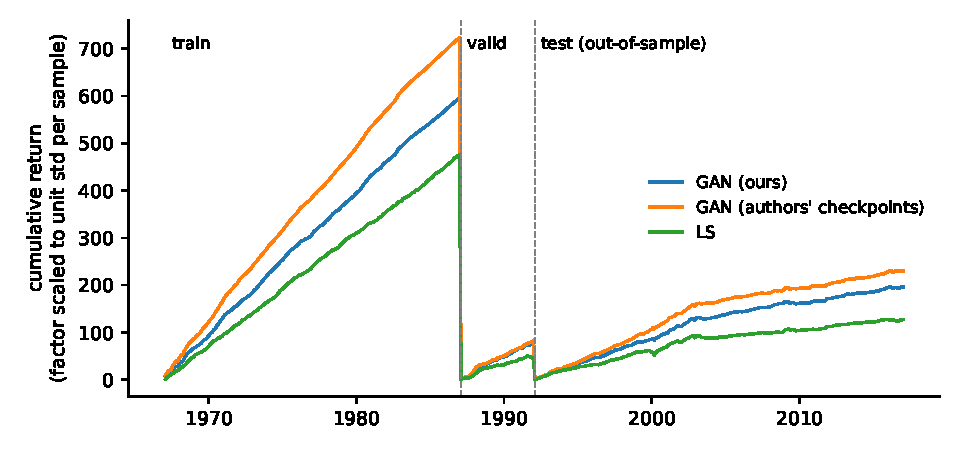
\includegraphics[width=0.44\textwidth]{../figures/fig_cumret.pdf}\hfill
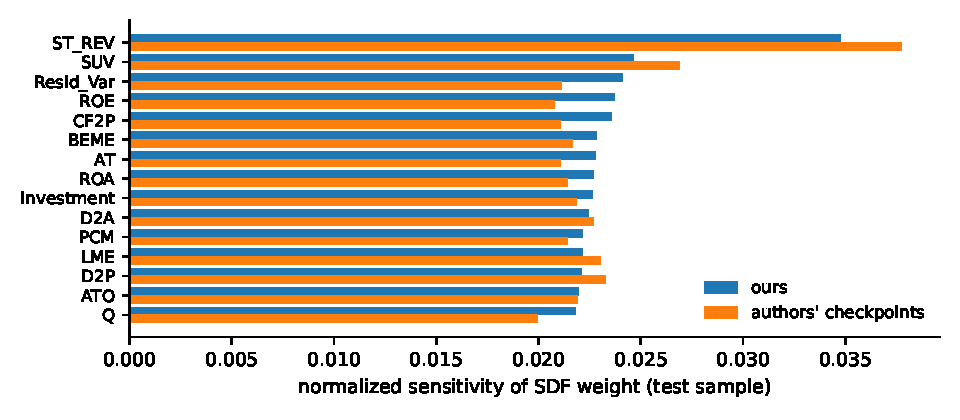
\includegraphics[width=0.44\textwidth]{../figures/fig_importance.pdf}
\end{center}
\vspace{-8pt}
{\small\emph{Left:} cumulative SDF-factor return, unit standard deviation within each sample. \emph{Right:} sensitivity of the
SDF weight to each characteristic (test sample), our ensemble vs the authors' checkpoints.}

\section{Challenges and how we dealt with them}
\begin{itemize}
\item \textbf{The official code does not run.} It is pinned to TensorFlow~1.12 / Python~3.6 (\texttt{tf.placeholder},
\texttt{tf.contrib}), which cannot be installed on Apple Silicon or any current Python. We re-implemented the model in
$\approx$250 lines of PyTorch from the paper's equations, using the TF source only to pin down undocumented details
(loss weights $T_i/\max T_j$, $L^1$ weight normalization, the 3-phase schedule, best-validation-Sharpe selection).
\item \textbf{Proving the re-implementation is faithful.} We read the authors' nine TF-1 checkpoints with TF2's
checkpoint reader and mapped them into our model. This needs the LSTM gate order (TF: $i,j,f,o$; PyTorch: $i,f,g,o$)
and TF's implicit $+1$ forget-gate bias. The ported ensemble gives test/validation Sharpe \authSRTe/\authSRVa{} vs
0.75/1.43 in Table~I. The authors also published their SDF-factor time series (\texttt{Data.xlsx}); it reproduces
Table~I to three decimals, and our ported factor has correlation \corrPortTe{} (test) / \corrPortTr{} (train) with it --
so the port is right and the released checkpoints are simply not the exact Table~I ensemble. Our own retrain has
correlation \corrOursTe{} (test) with the published factor.
\item \textbf{Unbalanced panel and LSTM state continuity.} Stocks enter and leave, so a $(T\times N)$ mask drives the SDF
sum, the per-stock moment means ($1/T_i$) and the loss weights; and the validation/test LSTM states must start from the
state at the end of the previous sample, not from zero -- resetting it silently destroys the out-of-sample numbers.
\item \textbf{Seed noise and model selection.} Individual seeds range from \trialTeMin{} to \trialTeMax{} test Sharpe
(validation \trialVaMin--\trialVaMax; the authors' own nine checkpoints: 0.45--0.62 test, 0.82--1.22 validation);
training Sharpe keeps rising while validation Sharpe plateaus (\texttt{fig\_training.pdf}). Best-validation-Sharpe
checkpoints plus an ensemble of \emph{weights} is what makes the result stable.
\item \textbf{Undocumented training-loop details.} The TF loop re-samples the adversary's instruments with dropout at
every step, selects checkpoints on the \emph{unnormalized} factor's validation Sharpe, never resets that tracker between
phases, and starts phase~3 with fresh Adam moments; none of this is in the paper. Our default run fixes $g$ after the
adversary step and selects on the normalized factor. Switching all four back (the ``TF-loop-faithful'' row) lifts
per-seed validation Sharpe to \tfVaMin--\tfVaMax{} (test \tfTeMin--\tfTeMax) and a \nTrialsTf{}-seed ensemble to
\tfSRTe{} out of sample -- these loop details, not the architecture, account for most of the gap to Table~I.
\item \textbf{Compute.} Full-batch training over 336k stock-months for 1\,280 epochs $\times$ 4 steps plus a validation
pass every epoch (the test sample is never touched during training): $\approx$35~min per seed on one CPU core,
$\approx$12~min on an Apple-silicon GPU (MPS); seeds were queued three at a time on the GPU.
\item \textbf{EV and XS-$R^2$ are not free.} They need the second-stage $\beta$ network described only in the code
(target $R^e_{t+1,i}F_{t+1}\times50$); the cross-sectional $R^2$ in Table~I is the $T_i$-weighted variant.
\end{itemize}

\section{Extensions}
\begin{itemize}
\item \textbf{Transaction costs (done).} With the paper's definition (Table~A.VII) the test-sample turnover of our
SDF portfolio is \turnLong{} for the long and \turnShort{} for the short leg (paper: 0.40 / 1.02); the short leg is
rebuilt almost entirely every month. Charging 10 / 25 / 50\,bp per unit of dollar turnover (\turnDollar{} per month)
cuts the test Sharpe from \ganSRTe{} to \srNetTen{} / \srNetTwentyFive{} / \srNetFifty{}. A cost-aware version would add a turnover penalty to the objective, which turns
the static weight map $\omega(I_t,I_{t,i})$ into a genuine control problem with the previous position as a state.
\item \textbf{Stability over time (done).} Test Sharpe is \srEarly{} in 1992--2004 vs \srLate{} in 2005--16 and
\srExGFC{} excluding 2008--09; worst month \maxLoss\%. The decay is the familiar post-publication erosion of
characteristic premia.
\item \textbf{Ablations run for free.} The unconditional model (no adversary) gives test Sharpe \uncSRTe{} and the linear
model \lsSRTe{}, isolating what the adversarial test assets and the nonlinearity buy.
\item \textbf{Reinforcement-learning reformulation.} $\omega(\cdot)$ is a policy mapping state $(h_t,I_{t,i})$ to actions;
maximizing the SDF Sharpe by policy gradient (actor--critic, with the adversary as a critic that finds mispriced test
assets) links the paper to the course and handles costs and constraints natively.
\item \textbf{Extend the sample and the state model.} Re-run on 2017--2025 data to measure out-of-sample decay; swap the
LSTM for a linear-Gaussian state-space model with a Kalman filter to test whether 4 nonlinear states beat 4 linear factors.
\end{itemize}
{\small Code in \texttt{replication/} (\texttt{gan\_sdf.py} is the model); data from \texttt{mpelger.people.stanford.edu/data-and-code}; paper arXiv:1904.00745.}
\end{document}
